\section[Xu hướng biến đổi một số tính chất]{Xu hướng biến đổi một số tính~chất của nguyên tử các~nguyên~tố trong một \newline chu kì và nhóm}
\vspace{1.25cm}
\begin{Muctieu}
	\begin{itemize}
		\item  Giải thích được xu hướng biến đổi bán kính nguyên tử trong một chu kì, trong một nhóm (nhóm A) (dựa theo lực hút tĩnh điện của hạt nhân với electron ngoài cùng và dựa theo số lớp electron tăng trong một nhóm theo chiểu từ trên xuống dưới).
		\item  Nhận xét và giải thích được xu hướng biến đổi độ âm điện và tính kim loại, phi kim của nguyên tử các nguyên tố trong một chu kì, trong một nhóm (nhóm A).
	\end{itemize}
\end{Muctieu}
\begin{kd}
	\immini{Hãy tưởng tượng bảng tuần hoàn giống như một lớp học lớn, nơi các học sinh được sắp xếp theo từng hàng và cột. Nếu chúng ta sắp xếp học sinh không theo thứ tự rõ ràng, việc quản lý và hiểu về từng nhóm học sinh sẽ trở nên rất khó khăn. Tương tự, việc sắp xếp các nguyên tố theo số hiệu nguyên tử giúp chúng ta tổ chức và hiểu rõ hơn về các tính chất của chúng.Hôm nay, chúng ta sẽ khám phá  xu hướng biến đổi một số tính chất như cấu hình e, kích thước nguyên tử, năng lượng ion hóa và tính axit-bazơ,$\ldots$ }{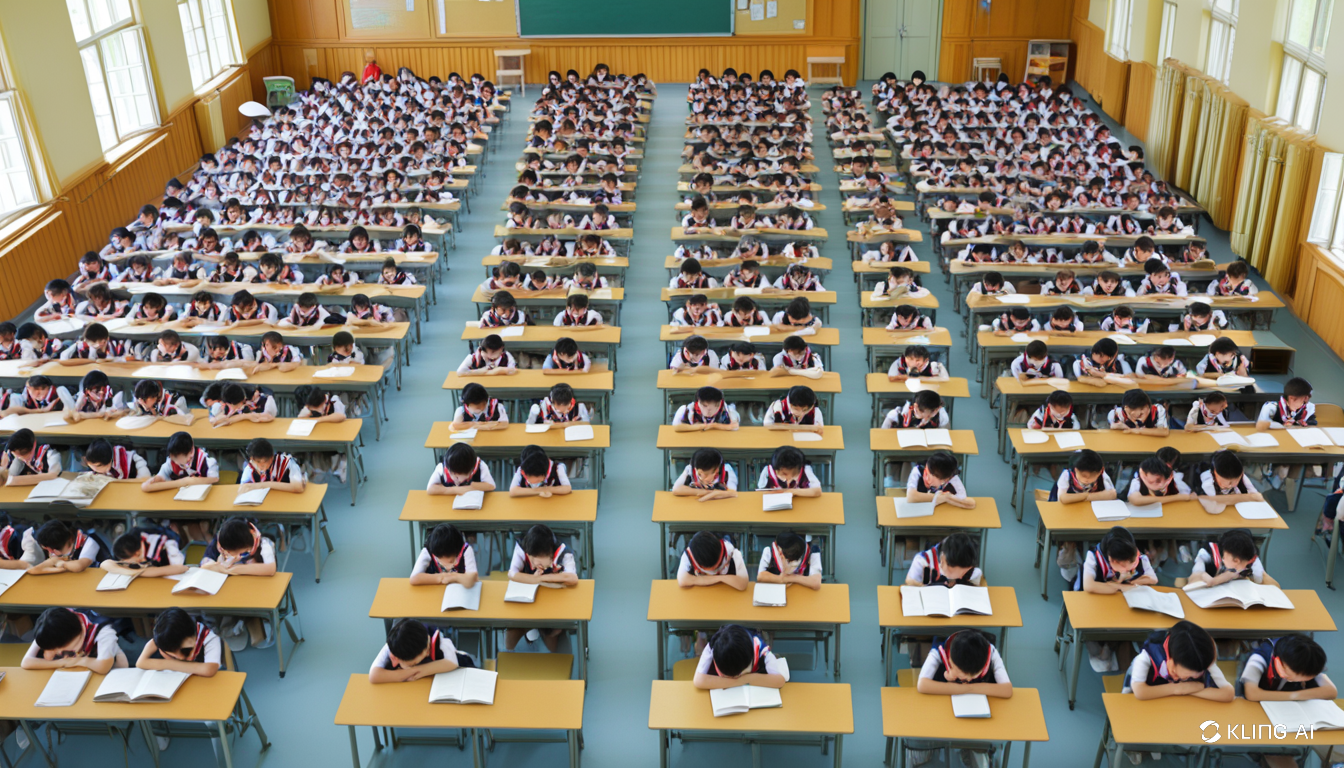
\includegraphics[width=6cm]{Images/anhhoahoc10/lophoc.png}}
\end{kd}
\subsection{Nội dung bài học}
		\subsubsection{Xu hướng biến đổi cấu hình electron lớp ngoài cùng nhóm A}
\vspace{0.25 cm}
\begin{tomtat}
	\begin{enumerate}
		\item Sau mỗi chu kì, cấu hình electron lớp ngoài cùng của nguyên tử các nguyên tố nhóm A được lặp đi lặp lại một cách tuần hoàn.\\
		Cụ thể số electron lớp ngoài cùng tăng dần từ 1 đến 8
		\begin{center}
			\begin{tabular}{|l*{8}{c}|}
				\hline
				\textbf{Nhóm} &IA&IIA&IIIA&IVA&VA&VIA&VIIA&VIIIA\\
				\textbf{Cấu hình e}& $ns^1$&$ns^2$&$ns^2np^1$&$ns^2np^2$&$ns^2np^3$&$ns^2np^4$&$ns^2np^5$&$ns^2np^6$\\
				\hline
			\end{tabular}
			\captionof{table}{Cấu hình e lớp ngoài cùng của các nguyên tử nguyên tố nhóm A}
		\end{center}
		\item Sự biến đổi tuần hoàn cấu hình electron lớp ngoài cùng của nguyên tử các nguyên tố khi điện tích hạt nhân tăng dần là nguyên nhân của sự biến đổi tuần hoàn về tính chất của các nguyên tố.
	\end{enumerate}
\end{tomtat}
\subsubsection{Xu hướng biến đổi bán kính nguyên tử}
\vspace{0.25cm}
\begin{hoivadap}
	Một hạt nhân có điện tich là +Z sẽ hút electron bằng một lực với độ lớn $\mathrm{F}=\mathrm{a} \tfrac{\mathrm{Z}}{\mathrm{r}^2}$, trong đó: r là khoảng cách từ hạt nhân tới electron, a lả một hằng số. Hãy cho biết:
	\begin{enumerate}[a)]
		\item  Điện tich hạt nhân càng lớn thì lực hút electron càng mạnh hay càng yếu?
		\item  Khoảng cách giữa electron và hạt nhân cảng lớn thì electron bị hạt nhân hút càng mạnh hay càng yếu?
	\end{enumerate}
\end{hoivadap}
\vspace{0.25cm}
\begin{tomtat}
	\begin{center}
		\resizebox{12cm}{!}{\begin{tikzpicture}[declare function={hsm=2.3;hsh=2.7;}]
				% Khai báo biến bán kính với đơn vị là 1/400
				\foreach \r/\n [count=\i] in {
					248/${}_{37}Rb$,215/${}_{38}Sr$,167/${}_{49}In$,140/${}_{50}Sn$,140/${}_{51}Sb$,142/${}_{52}Te$,133/${}_{53}I$,
					227/${}_{18}Ar$,197/${}_{20}Ca$,135/${}_{31}Ga$,122/${}_{32}Ge$,120/${}_{33}As$,119/${}_{34}Se$,114/${}_{35}Br$,
					186/${}_{11}Na$,160/${}_{12}Mg$,143/${}_{13}Al$,118/${}_{14}Si$,110/${}_{15}P$,103/${}_{16}S$,100/${}_{17}Cl$,
					152/${}_{3}Li$,112/${}_{4}Be$,85/${}_{5}B$,77/${}_{6}C$,75/${}_{7}N$,73/${}_{8}O$,72/${}_{9}F$
				} {
					% Tính toán vị trí x, y dựa trên chỉ số i
					\pgfmathsetmacro{\x}{hsm*(mod(\i-1,7) + 1)}
					\pgfmathsetmacro{\y}{hsh*(int((\i-1)/7) + 1)}
					\path (\x,\y) node[color=white,circle, ball color=\mauphu, minimum size={\r/4}, inner sep=0pt,anchor=south] (circle-\i){\n};
					\path (circle-\i.south) node[below] {\r};
				}
				\foreach \i [count=\c from 2] in{22,15,8,1} {
					\path (circle-\i) node [xshift=-1.5cm,font=\Large\bfseries](ck-\c){\c};
				}
				
				\foreach \i [count=\t from 1]  in{22,23,...,28} {
					\path (circle-\i.south) node [yshift=1.8cm,font=\Large\bfseries]{\MakeUppercase{\romannumeral\t} A};
				}
				\draw[-latex,line width=2pt,line cap=round,line join=round] ([xshift=-2cm]circle-22.north)--([xshift=-2cm]circle-1.south) node[pos=0.5,below,sloped,font=\bfseries\sffamily]{Chiều tăng của bán kính nguyên tử};
				
				\draw[-latex,line width=2pt,line cap=round,line join=round,shorten <=-0.8cm,shorten >=-0.8cm] ([yshift=-0.8cm]circle-1.south)--([yshift=-0.8cm]circle-7.south) node[pos=0.5,below,sloped,font=\bfseries\sffamily]{Chiều giảm của bán kính nguyên tử};
		\end{tikzpicture}}
		\captionof{figure}{Giá trị bán kính nguyên tử}
	\end{center}
	Xu hướng biến đổi bán kính nguyên tử:
	\begin{itemize}
		\item  Trong một chu kì, bán kính nguyên tử giảm theo chiều tăng dần của điện tích hạt nhân.
		\item  Trong một nhóm A , bán kính nguyên tử tăng theo chiều tăng dần của điện tích hạt nhân.
	\end{itemize}
\end{tomtat}
\begin{hoivadap}
	\begin{cauhoi}
		Giải thích xu hướng biến đổi bán kính
	\end{cauhoi}
	\loigiai{
		\begin{enumerate}
			\item Xu hướng biến đổi bán kính nguyên tử trong một chu kỳ (theo hàng ngang):
			\begin{itemize}
				\item  Khi đi từ trái sang phải trong một chu kỳ bán kính nguyên tử giảm dần.
				\item  Lý do:Khi di chuyển từ trái sang phải trong cùng một chu kỳ, số proton trong hạt nhân tăng lên, tức là điện tích hạt nhân tăng lên. Mặc khác số lớp electron không đổi, lực hút giữa hạt nhân (có điện tích dương) và các electron (có điện tích âm) mạnh hơn. Kết quả là các electron bị hút gần hơn về phía hạt nhân, làm cho bán kính nguyên tử giảm đi.
			\end{itemize}
			\item Xu hướng biến đổi bán kính nguyên tử trong một nhóm (theo cột dọc):
			\begin{itemize}
				\item  Khi đi từ trên xuống dưới trong một nhóm bán kính nguyên tử tăng dần.
				\item  Lý do:Khi di chuyển từ trên xuống dưới trong cùng một nhóm, số lớp electron tăng lên (mỗi nguyên tử mới có thêm một lớp electron so với nguyên tử phía trên nó). Mặc dù điện tích hạt nhân cũng tăng lên, nhưng sự gia tăng về số lượng lớp electron làm tăng khoảng cách giữa hạt nhân và electron ngoài cùng. Điều này làm giảm lực hút giữa hạt nhân và các electron ngoài cùng, do đó bán kính nguyên tử tăng lên.
			\end{itemize}
		\end{enumerate}
	}
\end{hoivadap}

\subsubsection{Xu hướng biến đổi độ âm điện}
\vspace{0.25cm}
\begin{tomtat}
	\textbf{Độ âm điện} của một nguyên tử đặc trưng cho khả năng hút electron của nguyên tử đó khi tạo thành liên kết hoá học.\\
	Xu hướng biến đổi độ âm điện theo chiều tăng dần của điện tích hạt nhân:
	\begin{itemize}
		\item Độ âm điện tăng từ trái qua phải trong một chu kì.
		\\
		Trong một chu kì, khi số electron lớp ngoài cùng tăng, điện tích hạt nhân tăng thì lực hút giữa hạt nhân với các electron lớp ngoài cùng tăng nên độ âm điện tăng.
		\item Độ âm điện giảm từ trên xuống dưới trong một nhóm A.
		\\
		Trong một nhóm A , khi số lớp electron tăng, lực hút giữa hạt nhân với các electron lớp ngoài cùng giảm nên độ âm điện giảm.
	\end{itemize}
\end{tomtat}
\subsubsection{Xu hướng biến đổi tính kim loại, tính phi kim}
\vspace{0.25cm}
\begin{tomtat}
	\Noibat{Khái niệm}
	\begin{itemize}
		\item \textbf{Tính kim loại} là tính chất của một nguyên tố mà nguyên tử của nó dễ nhường electron để trở thành ion dương. Nguyên tử của nguyên tố nào càng dễ nhường electron để trở thành ion dương, tính kim loại của nguyên tố đó càng mạnh.
		\item \textbf{Tính phi kim} là tính chất của một nguyên tố mà nguyên tử của nó dễ nhận electron để trở thành ion âm. Nguyên tử của nguyên tố nào càng dễ nhận electron để trở thành ion âm, tính phi kim của nguyên tố đó càng mạnh.
	\end{itemize}
	\Noibat{Xu hướng biến đổi}
	\begin{itemize}
		\item  \textbf{Trong một chu kì}, theo chiều tăng dần của điện tích hạt nhân, tính kim loại giảm dần và tính phi kim tăng dần. Do bán kính nguyên tử giảm, lực hút giữa hạt nhân với các electron lớp ngoài cùng tăng, dẫn đến khả năng nhường electron giảm nên tính kim loại giảm, khả năng nhận electron tăng nên tính phi kim tăng.
		\item  \textbf{Trong một nhóm A}, theo chiều tăng dần của điện tích hạt nhân, tính kim loại tăng dần và tính phi kim giảm dần. Tuy điện tích hạt nhân tăng dần, nhưng bán kính nguyên tử tăng nhanh hơn, lực hút giữa hạt nhân với các electron lớp ngoài cùng giảm dẫn đến khả năng nhường electron tăng nên tính kim loại tăng, khả năng nhận electron giảm nên tính phi kim giảm.
	\end{itemize}
\end{tomtat}
\subsection{Các dạng bài tập}
	%%%=============SOẠN EX===============%%%
\Opensolutionfile{ansex}[Ans/LGEX-H10C02B02-XHBDTC.tex]
\Opensolutionfile{ans}[Ans/Ans-H10C02B02-XHBDTC.tex]
%\tatloigiaiex
%\luuloigiaiex
\hienthiloigiaiex
\phan{Phần trắc nghiệm khách quam}
%%%=============EX_1=============%%%
\begin{ex}%[0H2N1-2]
	Trong cùng một chu kỳ, khi đi từ trái sang phải, cấu hình electron lớp ngoài cùng của các nguyên tố nhóm A có sự thay đổi như thế nào?
	\choice
	{\True Số electron lớp ngoài cùng tăng dần từ 1 đến 8}
	{Số electron lớp ngoài cùng giảm dần từ 8 về 1}
	{Số electron lớp ngoài cùng không đổi bằng số thứ tự chu kì}
	{Số electron lớp ngoài cùng tăng dần từ từ 1 đến 4 sau đó giảm dần từ 4 về 1}
	\loigiai{Trong một chu kỳ, khi đi từ trái sang phải, số electron lớp ngoài cùng của nguyên tử tăng dần từ 1 đến 8}
\end{ex}
%%%%=============EX_2=============%%%
\begin{ex}%[0H2N1-2]
	Trong một nhóm A, bán kính nguyên tử có xu hướng thay đổi như thế nào khi đi từ trên xuống dưới?
	\choice
	{Giảm dần}
	{\True Tăng dần}
	{Không thay đổi}
	{Tăng, sau đó giảm}
	\loigiai{Trong một nhóm A, bán kính nguyên tử tăng dần từ trên xuống dưới do số lớp electron tăng lên, làm giảm lực hút giữa hạt nhân và electron lớp ngoài cùng.}
\end{ex}
%%%%=============EX_3=============%%%
\begin{ex}%[0H2N1-2]
	Độ âm điện của các nguyên tố trong cùng một chu kỳ thay đổi như thế nào khi đi từ trái sang phải?
	\choice
	{Giảm dần}
	{Không thay đổi}
	{\True Tăng dần}
	{Tăng, sau đó giảm}
	\loigiai{Độ âm điện tăng dần từ trái sang phải trong cùng một chu kỳ sô lớp e không đổi , điện tích hạt nhân tăng, làm tăng lực hút đối với electron.}
\end{ex}
%%%=============EX_4=============%%%
\begin{ex}%[0H2H1-2]
	Nguyên tố nào sau đây có bán kính nguyên tử lớn nhất trong nhóm IA?
	\choice
	{Na}
	{K}
	{\True Cs}
	{Li}
	\loigiai{Trong nhóm IA, bán kính nguyên tử tăng từ trên xuống dưới do số lớp electron tăng lên. Cs có bán kính nguyên tử lớn nhất vì nằm ở dưới cùng của nhóm IA.}
\end{ex}
%%%=============EX_5=============%%%
\begin{ex}%[0H2H1-2]
	Trong chu kỳ 2, nguyên tố nào có độ âm điện cao nhất?
	\choice
	{Li}
	{Be}
	{O}
	{\True F}
	\loigiai{Trong chu kỳ 2, độ âm điện tăng dần từ trái sang phải. F có độ âm điện cao nhất với giá trị $3{,}98$.}
\end{ex}
%%%=============EX_6=============%%%
\begin{ex}%[0H2V1-2]
	Khi đi từ trên xuống dưới trong nhóm VIIA, tính chất hóa học của các nguyên tố thay đổi như thế nào?
	\choice
	{\True Tính oxi hóa giảm dần}
	{Tính oxi hóa tăng dần}
	{Tính khử giảm dần}
	{Tính khử không thay đổi}
	\loigiai{Trong nhóm VIIA, khi đi từ trên xuống dưới, tính oxi hóa của các nguyên tố giảm dần do bán kính nguyên tử tăng, làm giảm khả năng nhận electron.}
\end{ex}
%%%=============EX_7=============%%%
\begin{ex}%[0H2V1-2]
	Tính kim loại của các nguyên tố trong một chu kỳ có xu hướng thay đổi như thế nào khi đi từ trái sang phải?
	\choice
	{\True Giảm dần}
	{Tăng dần}
	{Không thay đổi}
	{Tăng, sau đó giảm}
	\loigiai{Trong một chu kỳ, tính kim loại giảm dần từ trái sang phải điện tích hạt nhân tăng số lớp electron không đổi do đó lực hút giưa hạt nhân và e tăng lên dẫn đến khả năng nhường e giảm}
\end{ex}
%%%=============EX_8=============%%%
\begin{ex}%[0H2V1-2]
	Nguyên tố nào sau đây có bán kính nguyên tử nhỏ nhất trong chu kỳ 3?
	\choice
	{Na}
	{Mg}
	{Al}
	{\True Cl}
	\loigiai{Trong chu kỳ 3, bán kính nguyên tử giảm dần từ trái sang phải. Cl có bán kính nhỏ nhất vì nó nằm gần cuối chu kỳ và có điện tích hạt nhân cao.}
\end{ex}
%%%=============EX_9=============%%%
\begin{ex}%[0H2H1-2]
	Tính chất nào sau đây là đúng khi so sánh các nguyên tố thuộc cùng một nhóm A?
	\choice
	{Các nguyên tố trong cùng nhóm có bán kính nguyên tử bằng nhau}
	{Các nguyên tố trong cùng nhóm có độ âm điện bằng nhau}
	{\True Các nguyên tố trong cùng nhóm có số electron hóa trị giống nhau}
	{Các nguyên tố trong cùng nhóm có cấu hình electron giống nhau}
	\loigiai{Các nguyên tố trong cùng nhóm A có số electron hóa trị giống nhau, điều này ảnh hưởng đến tính chất hóa học của chúng.}
\end{ex}
%%%=============EX_10=============%%%
\begin{ex}%[0H2H1-2]
	Tính kim loại của các nguyên tố trong cùng một nhóm A thay đổi như thế nào khi đi từ trên xuống dưới?
	\choice
	{Giảm dần}
	{\True Tăng dần}
	{Không thay đổi}
	{Tăng, sau đó giảm}
	\loigiai{Trong cùng một nhóm A, tính kim loại tăng dần từ trên xuống dưới do bán kính nguyên tử tăng, làm giảm lực hút giữa hạt nhân và electron lớp ngoài cùng, dễ dàng mất electron hơn.}
\end{ex}
%%%=============EX_11=============%%%
\begin{ex}%[0H2H1-2]
	Nguyên tố nào sau đây có tính kim loại mạnh nhất trong chu kỳ 4?
	\choice
	{\True K}
	{Ca}
	{Sc}
	{Ti}
	\loigiai{Trong chu kỳ 4, K là nguyên tố có tính kim loại mạnh nhất vì nó nằm ở đầu chu kỳ, có khả năng dễ dàng mất electron để tạo thành ion dương.}
\end{ex}
%%%=============EX_12=============%%%
\begin{ex}%[0H2H1-2]
	Độ âm điện của các nguyên tố trong nhóm VIA thay đổi như thế nào khi đi từ trên xuống dưới?
	\choice
	{\True Giảm dần}
	{Tăng dần}
	{Không thay đổi}
	{Tăng, sau đó giảm}
	\loigiai{Độ âm điện của các nguyên tố trong nhóm VIA giảm dần khi đi từ trên xuống dưới do bán kính nguyên tử tăng và khả năng hút electron của hạt nhân giảm.}
\end{ex}
%%%=============EX_13=============%%%
\begin{ex}%[0H2H1-2]
	Trong chu kỳ 3, nguyên tố nào sau đây có tính phi kim mạnh nhất?
	\choice
	{Na}
	{Mg}
	{Si}
	{\True Cl}
	\loigiai{Trong chu kỳ 3, tính phi kim tăng dần từ trái sang phải. Cl có tính phi kim mạnh nhất vì nó nắm ở cuối chu kì 3.}
\end{ex}
%%%=============EX_14=============%%%
\begin{ex}%[0H2H1-2]
	Nguyên tố nào sau đây thuộc nhóm VIIA và có bán kính nguyên tử lớn nhất?
	\choice
	{F}
	{Cl}
	{Br}
	{\True I}
	\loigiai{I (Iot) thuộc nhóm VIIA và có bán kính nguyên tử lớn nhất trong nhóm do số lớp electron nhiều nhất.}
\end{ex}
%%%=============EX_15=============%%%
\begin{ex}%[0H2H1-2]
	Cấu hình electron của các nguyên tố trong cùng nhóm IA có đặc điểm gì chung?
	\choice
	{Có số lớp electron giống nhau}
	{Có 1 lớp electron }
	{\True Có một electron ở lớp ngoài cùng}
	{Có số proton giống nhau}
	\loigiai{Các nguyên tố trong nhóm IA đều có một electron ở lớp ngoài cùng, dẫn đến tính chất hóa học tương tự nhau.}
\end{ex}
%%%=============EX_16=============%%%
\begin{ex}%[0H2H1-2]
	Trong nhóm IIA, nguyên tố nào có tính kim loại yếu nhất?
	\choice
	{\True Be}
	{Mg}
	{Ca}
	{Ba}
	\loigiai{Be có tính kim loại yếu nhất trong nhóm IIA vì nó nằm ở đầu nhóm, bán kính nguyên tử nhỏ và lực hút giữa hạt nhân với electron ngoài cùng mạnh hơn.}
\end{ex}
%%%=============EX_17=============%%%
\begin{ex}%[0H2H1-2]
	Nguyên tố nào sau đây thuộc chu kỳ 3 và có tính phi kim mạnh nhất?
	\choice
	{Na}
	{\True S}
	{Al}
	{P}
	\loigiai{S có tính phi kim mạnh nhất trong chu kỳ 3 do có độ âm điện cao hơn và khả năng nhận electron mạnh hơn.}
\end{ex}
%%%=============EX_18=============%%%
\begin{ex}%[0H2H1-2]
	Tính chất nào sau đây không thay đổi khi đi từ trái sang phải trong cùng một chu kỳ?
	\choice
	{\True Số lớp electron}
	{Độ âm điện}
	{Bán kính nguyên tử}
	{Tính kim loại}
	\loigiai{Số lớp electron không thay đổi khi đi từ trái sang phải trong cùng một chu kỳ, chỉ có số electron ngoài cùng và các tính chất liên quan thay đổi.}
\end{ex}
%%%=============EX_19=============%%%
\begin{ex}%[0H2H1-2]
	Trong nhóm VIIIA (nhóm khí hiếm), tính chất nào của các nguyên tố là giống nhau?
	\choice
	{Bán kính nguyên tử}
	{Khả năng phản ứng}
	{Số lớp electron}
	{\True Số electron hóa trị}
	\loigiai{Các nguyên tố trong nhóm VIIIA đều có số electron hóa trị bằng nhau (8 electron, trừ He có 2), làm cho chúng ổn định và ít phản ứng.}
\end{ex}
%%%=============EX_20=============%%%
\begin{ex}%[0H2H1-2]
	Trong nhóm IIIA, nguyên tố nào có tính phi kim yếu nhất?
	\choice
	{\True B}
	{Al}
	{Ga}
	{In}
	\loigiai{B có tính phi kim yếu nhất trong nhóm IIIA vì nó là nguyên tố đầu nhóm với bán kính nguyên tử nhỏ và lực hút electron mạnh hơn.}
\end{ex}
%%%=============EX_21=============%%%
\begin{ex}%[0H2H1-2]
	Nguyên tố nào sau đây có độ âm điện lớn nhất trong nhóm VIIA?
	\choice
	{Cl}
	{\True F}
	{Br}
	{I}
	\loigiai{F có độ âm điện lớn nhất trong nhóm VIIA do nằm ở đầu nhóm và có khả năng hút electron mạnh nhất.}
\end{ex}
%%%=============EX_22=============%%%
\begin{ex}%[0H2H1-2]
	Bán kính nguyên tử của các nguyên tố trong nhóm IIA thay đổi như thế nào khi đi từ trên xuống dưới?
	\choice
	{\True Tăng dần}
	{Giảm dần}
	{Không thay đổi}
	{Tăng, sau đó giảm}
	\loigiai{Trong nhóm IIA, bán kính nguyên tử tăng dần từ trên xuống dưới do có thêm các lớp electron mới, làm giảm lực hút giữa hạt nhân và electron ngoài cùng.}
\end{ex}
%%%%=============EX_23=============%%%
\begin{ex}%[0H2H1-2]
	Trong nhóm VIIIA, nguyên tố nào có bán kính nguyên tử lớn nhất?
	\choice
	{Ne}
	{Ar}
	{Kr}
	{\True Rn}
	\loigiai{Rn có bán kính nguyên tử lớn nhất trong nhóm VIIIA vì nó nằm ở dưới cùng của nhóm và có nhiều lớp electron nhất.}
\end{ex}
%%%=============EX_24=============%%%
\begin{ex}%[0H2H1-2]
	Trong chu kỳ 4, nguyên tố nào có bán kính nguyên tử lớn nhất?
	\choice
	{\True K}
	{ Rb}
	{Ca}
	{Sc}
	\loigiai{K có bán kính nguyên tử lớn nhất trong chu kỳ 4 do nó nằm ở đầu chu kỳ và có số lớp electron nhiều hơn các nguyên tố khác trong cùng chu kỳ.}
\end{ex}
%%%=============EX_25=============%%%
\begin{ex}%[0H2H1-2]
	Nguyên tố nào sau đây thuộc chu kỳ 3 và có bán kính nguyên tử nhỏ nhất?
	\choice
	{Na}
	{Mg}
	{Al}
	{\True Cl}
	\loigiai{Trong chu kỳ 3, bán kính nguyên tử giảm dần từ trái sang phải. Cl có bán kính nguyên tử nhỏ nhất vì nó có điện tích hạt nhân lớn nhất trong chu kỳ.}
\end{ex}
%%%=============EX_28=============%%%
\begin{ex}%[0H2H1-2]
	Nguyên tố nào sau đây thuộc chu kỳ 4 và có tính kim loại mạnh nhất?
	\choice
	{Sc}
	{Ti}
	{\True K}
	{Ca}
	\loigiai{K có tính kim loại mạnh nhất trong chu kỳ 4 vì nó có khả năng dễ dàng mất electron để tạo thành ion dương, điều này đặc trưng cho các kim loại mạnh.}
\end{ex}
%%%=============EX_29=============%%%
\begin{ex}%[0H2H1-2]
	Trong chu kỳ 2, nguyên tố nào có tính phi kim mạnh nhất?
	\choice
	{B}
	{N}
	{O}
	{\True F}
	\loigiai{F có tính phi kim mạnh nhất trong chu kỳ 2 vì nó có độ âm điện cao nhất, khả năng hút electron mạnh nhất, và dễ dàng nhận electron để đạt cấu hình bền vững.}
\end{ex}
%%%=============EX_30=============%%%
\begin{ex}%[0H2H1-2]
	Nguyên tố nào sau đây thuộc nhóm VIIA?
	\choice
	{Na}
	{Mg}
	{\True Cl}
	{K}
	\loigiai{Cl là nguyên tố thuộc nhóm VIIA, hay còn gọi là nhóm halogen. Na, Mg và K thuộc các nhóm khác nhau.}
\end{ex}
%%%=============EX_31=============%%%
\begin{ex}%[0H2H1-2]
	Phát biểu nào sau đây về các nguyên tố nhóm IIA là đúng?
	\choice
	{Các nguyên tố này đều là phi kim}
	{Các nguyên tố này có độ âm điện rất lớn}
	{Các nguyên tố này đều có bán kính nguyên tử nhỏ}
	{\True Các nguyên tố này đều có hai electron lớp ngoài cùng}
	\loigiai{Các nguyên tố nhóm IIA đều là kim loại và có hai electron ở lớp ngoài cùng. Độ âm điện của chúng không lớn và bán kính nguyên tử thay đổi tùy thuộc vào vị trí trong nhóm.}
\end{ex}
%%%=============EX_32=============%%%
\begin{ex}%[0H2H1-2]
	Trong một chu kỳ, theo chiều tăng của điện tích hạt nhân nguyên tử, bán kính nguyên tử:
	\choice
	{\True Giảm dần}
	{Tăng dần}
	{Không thay đổi}
	{Tăng rồi giảm}
	\loigiai{Bán kính nguyên tử giảm dần khi di chuyển từ trái sang phải trong một chu kỳ do lực hút của hạt nhân với các electron ngoài cùng tăng lên.}
\end{ex}

%%%=============EX_34=============%%%
\begin{ex}%[0H2H1-2]
	Phát biểu nào sau đây đúng với các nguyên tố thuộc nhóm VIA?
	\choice
	{Chúng đều là kim loại}
	{\True Chúng có xu hướng nhận thêm electron để đạt cấu hình bền vững}
	{Chúng có độ âm điện thấp}
	{Chúng có bán kính nguyên tử lớn nhất trong chu kỳ}
	\loigiai{Các nguyên tố nhóm VIA (như O, S) có tính phi kim mạnh và thường nhận thêm electron để đạt cấu hình bền vững.}
\end{ex}
%%%=============EX_35=============%%%
\begin{ex}%[0H2H1-2]
	Trong nhóm IA (kim loại kiềm), phát biểu nào sau đây là đúng?
	\choice
	{Các nguyên tố này đều có tính phi kim}
	{Chúng có độ âm điện rất lớn}
	{\True Chúng có bán kính nguyên tử lớn nhất trong chu kỳ}
	{Chúng có xu hướng nhận electron để trở thành anion}
	\loigiai{Các nguyên tố nhóm IA là kim loại và có bán kính nguyên tử lớn nhất trong chu kỳ. Chúng dễ dàng mất electron để tạo thành cation.}
\end{ex}
%%%=============EX_36=============%%%
\begin{ex}%[0H2V2-1]
	Nguyên tố X có số hiệu nguyên tử là 17. Phát biểu nào sau đây về X là đúng?
	\choice
	{X là kim loại kiềm}
	{\True X có thể tạo ra hợp chất với natri}
	{X là khí hiếm}
	{X có số electron ngoài cùng là 2}
	\loigiai{Nguyên tố X có số hiệu nguyên tử 17 là clo (Cl), một halogen. Nó có thể tạo hợp chất với natri để tạo ra muối ăn (NaCl).}
\end{ex}

%%%=============EX_39=============%%%
\begin{ex}%[0H2H1-2]
	Trong chu kỳ 2, phát biểu nào sau đây về các nguyên tố là đúng?
	\choice
	{Các nguyên tố đều là kim loại}
	{\True Tính phi kim tăng dần từ trái sang phải}
	{Bán kính nguyên tử tăng từ trái sang phải}
	{Tính kim loại tăng dần từ trái sang phải}
	\loigiai{Trong chu kỳ 2, tính phi kim tăng dần từ trái sang phải, và bán kính nguyên tử giảm dần do lực hút hạt nhân tăng.}
\end{ex}
%%%=============EX_40=============%%%
\begin{ex}%[0H2H1-2]
	Nguyên tố nào sau đây có độ âm điện lớn nhất trong nhóm VIA?
	\choice
	{S}
	{\True O}
	{Se}
	{Te}
	\loigiai{Oxy (O) có độ âm điện lớn nhất trong nhóm VIA, do nó có kích thước nguyên tử nhỏ nhất và điện tích hạt nhân cao nhất trong nhóm.}
\end{ex}
%%%%=============EX_41=============%%%
\begin{ex}%[0H2H1-2]
	Phát biểu nào sau đây về các nguyên tố thuộc nhóm IIIA là đúng?
	\choice
	{\True Chúng đều có 3 electron ở lớp ngoài cùng}
	{Chúng có tính kim loại mạnh nhất trong bảng tuần hoàn}
	{Chúng đều là phi kim}
	{Chúng có xu hướng nhận electron để tạo anion}
	\loigiai{Các nguyên tố nhóm IIIA đều có 3 electron ở lớp ngoài cùng, và chúng có tính chất của kim loại hoặc á kim.}
\end{ex}
%%%=============EX_42=============%%%
\begin{ex}%[0H2V1-2]
	Nguyên tố X thuộc chu kỳ 3 và có số hiệu nguyên tử là 16. Phát biểu nào sau đây về X là đúng?
	\choice
	{X là kim loại}
	{X có bán kính nguyên tử lớn nhất trong chu kỳ 3}
	{\True X có độ âm điện cao và là phi kim}
	{X có số electron lớp ngoài cùng là 2}
	\loigiai{Nguyên tố X là lưu huỳnh (S), thuộc nhóm VIA, là phi kim và có độ âm điện cao trong chu kỳ 3.}
\end{ex}
%%%=============EX_43=============%%%
\begin{ex}%[0H2H1-2]
	Trong nhóm VIIA, phát biểu nào sau đây là đúng?
	\choice
	{Các nguyên tố đều có bán kính nguyên tử lớn nhất trong chu kỳ}
	{\True Các nguyên tố đều có 7 electron lớp ngoài cùng}
	{Các nguyên tố đều có tính kim loại mạnh}
	{Các nguyên tố đều có độ âm điện nhỏ}
	\loigiai{Các nguyên tố nhóm VIIA đều có 7 electron ở lớp ngoài cùng và là những phi kim điển hình.}
\end{ex}

%%%=============EX_45=============%%%
\begin{ex}%[0H2H1-2]
	Nguyên tố Z có số hiệu nguyên tử là 20. Phát biểu nào sau đây về Z là đúng?
	\choice
	{\True Z là kim loại kiềm thổ và thuộc nhóm IIA}
	{Z là phi kim và có độ âm điện cao}
	{Z có bán kính nguyên tử nhỏ nhất trong chu kỳ}
	{Z có 1 electron lớp ngoài cùng}
	\loigiai{Nguyên tố Z là canxi (Ca), thuộc nhóm IIA, là kim loại kiềm thổ với 2 electron ở lớp ngoài cùng.}
\end{ex}
%%%=============EX_46=============%%%
\begin{ex}%[0H2H1-2]
	Dãy nguyên tố nào sau đây sắp xếp theo chiều tăng dần của năng lượng ion hóa?
	\choice
	{K, Ca, Mg, Na}
	{Mg, Na, K, Ca}
	{\True $\mathrm{Na}, \mathrm{Mg}, \mathrm{Ca}, \mathrm{K}$}
	{$\mathrm{Ca}, \mathrm{K}, \mathrm{Mg}, \mathrm{Na}$}
	\loigiai{Năng lượng ion hóa tăng dần từ trái sang phải trong một chu kì và giảm dần từ trên xuống dưới trong một nhóm.}
\end{ex}
%%%=============EX_47=============%%%
\begin{ex}%[0H2H1-2]
	Nguyên tử của nguyên tố nào có bán kính nhỏ nhất trong các nguyên tử sau đây?
	\choice
	{Si}
	{N}
	{\True O}
	{P}
	\loigiai{Bán kính nguyên tử giảm dần từ trái sang phải trong một chu kì. Nguyên tố có bán kính nhỏ nhất trong các nguyên tử đã cho là oxi (O).}
\end{ex}

%%%=============EX_49=============%%%
\begin{ex}%[0H2H1-2]
	Nguyên tử của nguyên tố nào sau đây có độ âm điện nhỏ nhất? Nguyên tố này thường được sử dụng trong chế tạo pin và năng lượng hạt nhân.
	\choice
	{Boron}
	{\True Lithium}
	{Carbon}
	{Phosphorus}
	\loigiai{Độ âm điện nhỏ nhất trong các nguyên tử đã cho là của nguyên tố lithium (Li).}
\end{ex}
%%%=============EX_50=============%%%

%%%=============EX_51=============%%%
\begin{ex}%[0H2H1-2]
	Nguyên tử của nguyên tố nào sau đây có tính phi kim mạnh nhất? Nguyên tố này được sử dụng để làm chất tẩy rửa và bảo vệ đồ vật khỏi sự ăn mòn.
	\choice
	{Chlorine}
	{Bromine}
	{\True Fluorine}
	{Iodine}
	\loigiai{Fluorine (F) là nguyên tố có tính phi kim mạnh nhất trong các nguyên tố đã cho.}
\end{ex}
%%%=============EX_54=============%%%
\begin{ex}%[0H2H2-1]
	Cho các nguyên tố $A, B, C$ với số hiệu nguyên tử lần lượt là $5, 13, 19$. Phát biểu nào sau đây là đúng?
	\choice
	{Các nguyên tố này đều nằm trong cùng một chu kì}
	{\True Thứ tự tăng dần tính kim loại là: $A, B, C$}
	{Các nguyên tố này đều thuộc nhóm chính}
	{Thứ tự tăng dần độ âm điện là: $C, B, A$}
	\loigiai{Thứ tự tăng dần tính kim loại đúng là $A, B, C$ với $A$ là boron, $B$ là aluminium và $C$ là kali.}
\end{ex}

\Closesolutionfile{ans}
\Closesolutionfile{ansex}
%\bangdapan{Ans-H10C02B02-XHBDTC.tex}

\phan{Phần trắc nghiệm đúng sai}
%%%=============SOẠN EXTF===============%%%
\Opensolutionfile{ansex}[Ans/LGTF-H10C02B02-XHBDTC.tex]
\Opensolutionfile{ansbook}[Ansbook/AnsTF-H10C02B02-XHBDTC.tex]
\Opensolutionfile{ans}[Ans/Tempt-H10C02B02-XHBDTC.tex]
\LGexTF
%%%=============EX_1=============%%%
\begin{ex}%[0H2H1-2]
	Trong chu kỳ, bán kính nguyên tử tăng khi
	\choiceTF[t]
	{Di chuyển từ trái sang phải}
	{\True Lực hút của hạt nhân và electron giảm}
	{\True Tăng số lớp electron}
	{Tăng điện tích hạt nhân}
	\loigiai{Bán kính nguyên tử tăng khi di chuyển từ phải sang trái trong chu kỳ do lực hút hạt nhân yếu hơn, và khi tăng số lớp electron.}
\end{ex}

%%%=============EX_2=============%%%
\begin{ex}%[0H2H1-2]
	Trong cùng một nhóm A của bảng tuần hoàn
	\choiceTF[t]
	{Bán kính nguyên tử giảm khi di chuyển từ trên xuống dưới}
	{\True Bán kính nguyên tử tăng khi di chuyển từ trên xuống dưới}
	{Tính kim loại giảm khi di chuyển từ trên xuống dưới}
	{\True Tính kim loại tăng khi di chuyển từ trên xuống dưới}
	\loigiai{Trong cùng một nhóm A, bán kính nguyên tử tăng và tính kim loại tăng khi di chuyển từ trên xuống dưới do có thêm lớp electron.}
\end{ex}
%
%%%=============EX_3=============%%%
\begin{ex}%[0H2H1-2]
	Độ âm điện của các nguyên tố 
	\choiceTF[t]
	{\True Tăng dần từ trái sang phải}
	{\True là đại lượng đặc trưng cho khả năng hút electron}
	{Không thay đổi trong cùng một nhóm}
	{Tăng dần từ trên xuống dưới}
	\loigiai{Độ âm điện tăng dần từ trái sang phải trong chu kỳ do tăng điện tích hạt nhân, và không thay đổi trong cùng một nhóm.}
\end{ex}
%
%%%=============EX_4=============%%%
\begin{ex}%[0H2H1-2]
	Trong nhóm IIA của bảng tuần hoàn
	\choiceTF[t]
	{\True Tính kim loại tăng từ Be đến Ba}
	{Độ âm điện tăng từ Be đến Ba}
	{\True Bán kính nguyên tử tăng từ Be đến Ba}
	{Tính phi kim tăng từ Be đến Ba}
	\loigiai{Trong nhóm IIA, tính kim loại và bán kính nguyên tử tăng từ Be đến Ba do có thêm lớp electron. Độ âm điện và tính phi kim giảm.}
\end{ex}

%%%=============EX_5=============%%%
\begin{ex}%[0H2H1-2]
	Các nguyên tố trong cùng một chu kỳ có:
	\choiceTF[t]
	{\True Số lớp electron bằng nhau}
	{\True Tính kim loại giảm dần từ trái sang phải}
	{\True Độ âm điện tăng dần từ trái sang phải}
	{Số electron hóa trị bằng nhau}
	\loigiai{Các nguyên tố trong cùng một chu kỳ có số lớp electron bằng nhau, và tính kim loại giảm dần từ trái sang phải. Độ âm điện tăng dần.}
\end{ex}
%
%%%=============EX_6=============%%%
\begin{ex}%[0H2H1-2]
	Nguyên tố thuộc nhóm VIIA (Halogen)
	\choiceTF[t]
	{Có tính kim loại mạnh}
	{\True Có độ âm điện cao}
	{\True Dễ dàng nhận electron để đạt cấu hình bền vững}
	{Có bán kính nguyên tử lớn nhất trong chu kỳ}
	\loigiai{Các nguyên tố Halogen có độ âm điện cao và dễ dàng nhận electron, nhưng không có tính kim loại mạnh và không có bán kính nguyên tử lớn nhất trong chu kỳ.}
\end{ex}

%%%=============EX_8=============%%%
\begin{ex}%[0H2H1-2]
	Các nguyên tố trong nhóm IA (kim loại kiềm)
	\choiceTF[t]
	{\True Có tính kim loại mạnh}
	{\True Dễ dàng mất electron để tạo ion dương}
	{Có độ âm điện cao}
	{\True Bán kính nguyên tử tăng từ trên xuống dưới}
	\loigiai{Các nguyên tố nhóm IA có tính kim loại mạnh, dễ mất electron và có bán kính nguyên tử tăng từ trên xuống dưới. Độ âm điện của chúng thấp.}
\end{ex}

%%%=============EX_9=============%%%
\begin{ex}%[0H2H1-2]
	Trong cùng một chu kỳ của bảng tuần hoàn
	\choiceTF[t]
	{\True Độ âm điện tăng dần từ trái sang phải}
	{\True Tính phi kim tăng dần từ trái sang phải}
	{Bán kính nguyên tử tăng từ trái sang phải}
	{Tính kim loại tăng từ trái sang phải}
	\loigiai{Trong cùng một chu kỳ, độ âm điện và tính phi kim tăng từ trái sang phải, trong khi bán kính nguyên tử và tính kim loại giảm.}
\end{ex}

%%%=============EX_10=============%%%
\begin{ex}%[0H2H1-2]
	Nguyên tố thuộc chu kỳ 3
	\choiceTF[t]
	{\True Có số lớp electron bằng nhau}
	{\True Tính phi kim tăng từ trái sang phải}
	{Bán kính nguyên tử tăng từ trái sang phải}
	{Tính kim loại tăng từ trái sang phải}
	\loigiai{Trong chu kỳ 3, các nguyên tố có số lớp electron bằng nhau, và tính phi kim tăng từ trái sang phải, trong khi bán kính nguyên tử và tính kim loại giảm.}
\end{ex}

%%%=============EX_12=============%%%
\begin{ex}%[0H2N1-2]
	Trong nhóm VIIA (Halogen)
	\choiceTF[t]
	{\True Độ âm điện giảm từ trên xuống dưới}
	{Bán kính nguyên tử giảm từ trên xuống dưới}
	{\True Tính phi kim giảm từ trên xuống dưới}
	{\True có 7 lelectron ở lớp ngoài cùng}
	\loigiai{Trong nhóm VIIA, độ âm điện và tính phi kim giảm từ trên xuống dưới, trong khi bán kính nguyên tử  tăng.Các nguyên tố đều có 7 electron ở lớp ngoài cùng.}
\end{ex}

%%%=============EX_13=============%%%
\begin{ex}%[0H2H1-2]
	Các nguyên tố thuộc nhóm IIIA
	\choiceTF[t]
	{\True Có bán kính nguyên tử tăng từ trên xuống dưới}
	{Có tính phi kim mạnh nhất trong nhóm}
	{Có độ âm điện cao nhất trong bảng tuần hoàn}
	{\True Có số lớp electron tăng từ trên xuống dưới}
	\loigiai{Các nguyên tố nhóm IIIA có bán kính nguyên tử và số lớp electron tăng từ trên xuống dưới, nhưng không có tính phi kim mạnh và độ âm điện cao nhất.}
\end{ex}
%
%%%=============EX_14=============%%%
\begin{ex}%[0H2H1-2]
	Trong chu kỳ 4 của bảng tuần hoàn
	\choiceTF[t]
	{\True Các nguyên tố có tính kim loại mạnh nhất ở đầu chu kỳ}
	{\True Bán kính nguyên tử giảm dần từ trái sang phải}
	{\True Độ âm điện tăng dần từ trái sang phải}
	{Tính phi kim mạnh nhất ở đầu chu kỳ}
	\loigiai{Trong chu kỳ 4, bán kính nguyên tử giảm dần và độ âm điện tăng dần từ trái sang phải. Tính kim loại mạnh nhất ở đầu chu kỳ}
\end{ex}
%
%%%=============EX_15=============%%%
\begin{ex}%[0H2H1-2]
	Các nguyên tố thuộc nhóm IVA (Carbon)
	\choiceTF[t]
	{\True Có số electron hóa trị bằng nhau}
	{ Có tính phi kim mạnh nhất ở đầu nhóm}
	{\True Tính kim loại tăng từ trên xuống dưới}
	{Độ âm điện tăng từ trên xuống dưới}
	\loigiai{Các nguyên tố nhóm IVA có số electron hóa trị bằng nhau và tính phi kim mạnh nhất ở đầu nhóm, tính kim loại tăng từ trên xuống dưới, trong khi độ âm điện giảm.}
\end{ex}
%
%
%%%=============EX_16=============%%%
\begin{ex}%[0H2H1-2]
	Xu hướng biến đổi bán kính nguyên tử trong cùng một chu kì từ trái sang phải là:
	\choiceTF[t]
	{\True Giảm dần do lực hút giữa hạt nhân và electron tăng dần.}
	{Tăng dần do số lượng electron trong cùng lớp vỏ tăng.}
	{Không đổi vì số lớp electron không thay đổi.}
	{\True Giảm mạnh ở nhóm cuối cùng do tính phi kim cao.}
	\loigiai{Trong cùng một chu kì, bán kính nguyên tử giảm dần từ trái sang phải do lực hút giữa hạt nhân và electron tăng dần khi số proton tăng.}
\end{ex}

%%%=============EX_17=============%%%
\begin{ex}%[0H2H1-2]
	Trong cùng một nhóm, bán kính nguyên tử:
	\choiceTF[t]
	{\True Tăng dần từ trên xuống dưới.}
	{Giảm dần từ trên xuống dưới.}
	{Không đổi vì số lượng lớp vỏ electron không thay đổi.}
	{\True Tăng nhẹ ở các nguyên tố phi kim.}
	\loigiai{Trong cùng một nhóm, bán kính nguyên tử tăng dần từ trên xuống dưới do số lớp vỏ electron tăng.}
\end{ex}
%%%%=============EX_18=============%%%
\begin{ex}%[0H2H1-2]
	Cho các phát biểu về  tính phi kim
	\choiceTF[t]
	{\True Giảm dần từ trên xuống dưới.}
	{\True là tính dễ nhận electron của nguyên tử nguyên tố đó}
	{\True Tăng dần từ trái sang phải.}
	{Ban đầu tăng rồi sau đó giảm dần trong một chu kì}
	\loigiai{Trong cùng một nhóm, tính phi kim giảm dần từ trên xuống dưới do bán kính nguyên tử tăng làm giảm khả năng nhận electron.Trong cùng chu kì bán kính nguyên tử giảm làm tăng khả năng nhận thêm electron.}
\end{ex}
\Closesolutionfile{ans}
\Closesolutionfile{ansbook}
\Closesolutionfile{ansex}
%\bangdapanTF{AnsTF-H10C02B02-XHBDTC.tex}


\phan{Phần tự luận}
%%%=============SOẠN BT===============%%%
\Opensolutionfile{ansbth}[Ans/LGBT-H10C02B02-XHBDTC.tex]
\Opensolutionfile{ansbt}[Ans/AnsBT-H10C02B02-XHBDTC.tex]
\hienthiloigiaibt
%%%==============Bai_BT1==============%%%
\begin{bt}%[0H2V2-1]
	Cho các nguyên tố sau: $\mathrm{B} (Z=5), \mathrm{N} (Z=7), \mathrm{O} (Z=8), \mathrm{F} (Z=9)$.
	Hãy sắp xếp các nguyên tố trên theo chiều tăng dần bán kính nguyên tử.
	\loigiai{Các nguyên tố trên đều thuộc chu kì 2 do đó theo chiều tăng dần của điện tích hạt nhân bán kính nguyên tử giảm do đó trật tự sắp xếp theo chiều bán kính tăng sẽ là: $\mathrm{F} < \mathrm{O} < \mathrm{N} < \mathrm{B}$.}
\end{bt}
%%%%==============HetBai_BT1==============%%%

%%%==============Bai_BT2==============%%%
\begin{bt}
	Cho các nguyên tố $X (Z=12), Y (Z=15), Z (Z=16), T (Z=17)$. 
	\begin{enumerate}
		\item Xác định vị trí của các nguyên tố đó trong bảng tuần hoàn.
		\item Xếp các nguyên tố đó theo thứ tự độ âm điện tăng dần.
	\end{enumerate}
	\loigiai{
		\begin{enumerate}
			\item $X$ là $\mathrm{Mg}$ (nhóm IIA), $Y$ là $\mathrm{P}$ (nhóm VA), $Z$ là $\mathrm{S}$ (nhóm VIA), $T$ là $\mathrm{Cl}$ (nhóm VIIA).
			\item Thứ tự độ âm điện tăng dần là: $X < Y < Z < T$ (vì độ âm điện tăng dần từ trái sang phải trong chu kỳ và từ dưới lên trên trong nhóm). 
		\end{enumerate}
	}
\end{bt}
%%%%==============HetBai_BT2==============%%%
%
%%%%==============Bai_BT3==============%%%
%\begin{bt}
%	Cho các nguyên tố thuộc nhóm VIA: $\mathrm{O} (Z=8)$, $\mathrm{S} (Z=16)$, $\mathrm{Se} (Z=34)$, $\mathrm{Te} (Z=52)$. 
%	\begin{enumerate}
%		\item Sắp xếp các nguyên tố theo thứ tự bán kính nguyên tử tăng dần.
%		\item Sắp xếp các nguyên tố theo thứ tự độ âm điện giảm dần.
%	\end{enumerate}
%	\loigiai{
%		\begin{enumerate}
%			\item Thứ tự bán kính nguyên tử tăng dần là: $\mathrm{O} < \mathrm{S} < \mathrm{Se} < \mathrm{Te}$ (bán kính nguyên tử tăng khi di chuyển xuống nhóm).
%			\item Thứ tự độ âm điện giảm dần là: $\mathrm{O} > \mathrm{S} > \mathrm{Se} > \mathrm{Te}$ (độ âm điện giảm khi di chuyển xuống nhóm). 
%		\end{enumerate}
%	}
%\end{bt}
%%%%==============HetBai_BT3==============%%%
%
%%%%==============Bai_BT4==============%%%
%\begin{bt}
%	Cho các nguyên tố $X (Z=6), Y (Z=8), Z (Z=14)$.
%	\begin{enumerate}
%		\item Xác định vị trí của các nguyên tố đó trong bảng tuần hoàn.
%		\item Xếp các nguyên tố đó theo thứ tự độ âm điện giảm dần.
%		\item Xếp các nguyên tố đó theo thứ tự bán kính nguyên tử tăng dần.
%		\item Xếp các nguyên tố đó theo thứ tự tính phi kim tăng dần.
%	\end{enumerate}
%	\loigiai{
%		\begin{enumerate}
%			\item $X$ là $\mathrm{C}$ (nhóm IVA), $Y$ là $\mathrm{O}$ (nhóm VIA), $Z$ là $\mathrm{Si}$ (nhóm IVA).
%			\item Thứ tự độ âm điện giảm dần là: $Y > X > Z$ (O có độ âm điện lớn nhất, sau đó đến C và Si).
%			\item Thứ tự bán kính nguyên tử tăng dần là: $Y < X < Z$ (bán kính tăng dần khi di chuyển xuống nhóm).
%			\item Thứ tự tính phi kim tăng dần là: $Z < X < Y$ (tính phi kim tăng dần từ trái sang phải trong chu kỳ).
%		\end{enumerate}
%	}
%\end{bt}
%%%%==============HetBai_BT4==============%%%
%
%%%%==============Bai_BT5==============%%%
%\begin{bt}
%	Cho các nguyên tố $X (Z=11), Y (Z=13), Z (Z=19)$.
%	\begin{enumerate}
%		\item Xác định vị trí của các nguyên tố đó trong bảng tuần hoàn.
%		\item Xếp các nguyên tố đó theo thứ tự bán kính nguyên tử giảm dần.
%		\item Gán các giá trị độ âm điện $(0,82; 1,31$ và 0,93$)$ cho $X, Y, Z$.
%		\item Xếp các nguyên tố đó theo thứ tự tính kim loại giảm dần.
%	\end{enumerate}
%	\loigiai{
%		\begin{enumerate}
%			\item $X$ là $\mathrm{Na}$ (nhóm IA), $Y$ là $\mathrm{Al}$ (nhóm IIIA), $Z$ là $\mathrm{K}$ (nhóm IA).
%			\item Thứ tự bán kính nguyên tử giảm dần là: $Z > X > Y$ (bán kính nguyên tử giảm dần từ trái sang phải trong chu kỳ).
%			\item Độ âm điện: $X = 0,82$, $Y = 1,31$, $Z = 0,93$.
%			\item Thứ tự tính kim loại giảm dần là: $Z > X > Y$ (tính kim loại giảm dần từ trái sang phải trong chu kỳ). 
%		\end{enumerate}
%	}
%\end{bt}
%%%%==============HetBai_BT5==============%%%
%
%%%%==============Bai_BT6==============%%%
%\begin{bt}
%	Cho các nguyên tố $\mathrm{F} (Z=9)$, $\mathrm{Cl} (Z=17)$, $\mathrm{Br} (Z=35)$ và $\mathrm{I} (Z=53)$.
%	\begin{enumerate}
%		\item Xếp các nguyên tố đó theo thứ tự độ âm điện giảm dần.
%		\item Xếp các nguyên tố đó theo thứ tự bán kính nguyên tử tăng dần.
%	\end{enumerate}
%	\loigiai{
%		\begin{enumerate}
%			\item Thứ tự độ âm điện giảm dần là: $\mathrm{F} > \mathrm{Cl} > \mathrm{Br} > \mathrm{I}$ (độ âm điện giảm khi di chuyển xuống nhóm).
%			\item Thứ tự bán kính nguyên tử tăng dần là: $\mathrm{F} < \mathrm{Cl} < \mathrm{Br} < \mathrm{I}$ (bán kính nguyên tử tăng khi di chuyển xuống nhóm). 
%		\end{enumerate}
%	}
%\end{bt}
%%%%==============HetBai_BT6==============%%%
%
%%%%==============Bai_BT7==============%%%
%\begin{bt}
%	Cho các nguyên tố $\mathrm{Li} (Z=3)$, $\mathrm{Be} (Z=4)$, $\mathrm{B} (Z=5)$ và $\mathrm{C} (Z=6)$.
%	\begin{enumerate}
%		\item Sắp xếp các nguyên tố theo thứ tự bán kính nguyên tử tăng dần.
%		\item Sắp xếp các nguyên tố theo thứ tự độ âm điện giảm dần.
%	\end{enumerate}
%	\loigiai{
%		\begin{enumerate}
%			\item Thứ tự bán kính nguyên tử tăng dần là: $\mathrm{C} < \mathrm{B} < \mathrm{Be} < \mathrm{Li}$ (bán kính nguyên tử giảm khi di chuyển từ trái sang phải trong một chu kỳ).
%			\item Thứ tự độ âm điện giảm dần là: $\mathrm{C} > \mathrm{B} > \mathrm{Be} > \mathrm{Li}$ (độ âm điện tăng khi di chuyển từ trái sang phải trong một chu kỳ). 
%		\end{enumerate}
%	}
%\end{bt}
%%%%==============HetBai_BT7==============%%%
%
%%%%==============Bai_BT8==============%%%
%\begin{bt}
%	Cho các nguyên tố $\mathrm{Na} (Z=11)$, $\mathrm{Mg} (Z=12)$, $\mathrm{Al} (Z=13)$ và $\mathrm{Si} (Z=14)$.
%	\begin{enumerate}
%		\item Xếp các nguyên tố đó theo thứ tự bán kính nguyên tử giảm dần.
%		\item Xếp các nguyên tố đó theo thứ tự tính kim loại giảm dần.
%	\end{enumerate}
%	\loigiai{
%		\begin{enumerate}
%			\item Thứ tự bán kính nguyên tử giảm dần là: $\mathrm{Na} > \mathrm{Mg} > \mathrm{Al} > \mathrm{Si}$ (bán kính nguyên tử giảm khi di chuyển từ trái sang phải trong một chu kỳ).
%			\item Thứ tự tính kim loại giảm dần là: $\mathrm{Na} > \mathrm{Mg} > \mathrm{Al} > \mathrm{Si}$ (tính kim loại giảm khi di chuyển từ trái sang phải trong một chu kỳ). 
%		\end{enumerate}
%	}
%\end{bt}
%%%%==============HetBai_BT8==============%%%
%
%%%%==============Bai_BT9==============%%%
%\begin{bt}
%	Cho các nguyên tố $\mathrm{H} (Z=1)$, $\mathrm{He} (Z=2)$, $\mathrm{Li} (Z=3)$ và $\mathrm{Be} (Z=4)$.
%	\begin{enumerate}
%		\item Sắp xếp các nguyên tố theo thứ tự độ âm điện tăng dần.
%		\item Sắp xếp các nguyên tố theo thứ tự bán kính nguyên tử giảm dần.
%	\end{enumerate}
%	\loigiai{
%		\begin{enumerate}
%			\item Thứ tự độ âm điện tăng dần là: $\mathrm{Be} < \mathrm{Li} < \mathrm{H} < \mathrm{He}$ (độ âm điện tăng dần từ trái sang phải trong chu kỳ, với H và He ở đầu chu kỳ có độ âm điện lớn hơn).
%			\item Thứ tự bán kính nguyên tử giảm dần là: $\mathrm{Li} > \mathrm{Be} > \mathrm{H} > \mathrm{He}$ (bán kính nguyên tử giảm dần từ trái sang phải trong một chu kỳ). 
%		\end{enumerate}
%	}
%\end{bt}
%%%%==============HetBai_BT9==============%%%
%
%%%%==============Bai_BT10==============%%%
%\begin{bt}
%	Cho các nguyên tố $\mathrm{K} (Z=19)$, $\mathrm{Ca} (Z=20)$, $\mathrm{Sc} (Z=21)$ và $\mathrm{Ti} (Z=22)$.
%	\begin{enumerate}
%		\item Xếp các nguyên tố đó theo thứ tự bán kính nguyên tử tăng dần.
%		\item Xếp các nguyên tố đó theo thứ tự độ âm điện giảm dần.
%	\end{enumerate}
%	\loigiai{
%		\begin{enumerate}
%			\item Thứ tự bán kính nguyên tử tăng dần là: $\mathrm{Ti} < \mathrm{Sc} < \mathrm{Ca} < \mathrm{K}$ (bán kính nguyên tử giảm dần khi di chuyển từ trái sang phải trong một chu kỳ).
%			\item Thứ tự độ âm điện giảm dần là: $\mathrm{K} < \mathrm{Ca} < \mathrm{Sc} < \mathrm{Ti}$ (độ âm điện giảm dần khi di chuyển từ trái sang phải trong một chu kỳ).
%		\end{enumerate}
%	}
%\end{bt}
%%%%==============HetBai_BT10==============%%%
%
%%%%==============Bai_BT11==============%%%
%\begin{bt}
%	Cho các nguyên tố $\mathrm{P} (Z=15)$, $\mathrm{S} (Z=16)$, $\mathrm{Cl} (Z=17)$ và $\mathrm{Br} (Z=35)$.
%	\begin{enumerate}
%		\item Xếp các nguyên tố đó theo thứ tự tính phi kim tăng dần.
%		\item Xếp các nguyên tố đó theo thứ tự bán kính nguyên tử tăng dần.
%	\end{enumerate}
%	\loigiai{
%		\begin{enumerate}
%			\item Thứ tự tính phi kim tăng dần là: $\mathrm{P} < \mathrm{S} < \mathrm{Cl} < \mathrm{Br}$ (tính phi kim tăng dần khi di chuyển xuống nhóm).
%			\item Thứ tự bán kính nguyên tử tăng dần là: $\mathrm{Cl} < \mathrm{Br} < \mathrm{S} < \mathrm{P}$ (bán kính nguyên tử tăng dần khi di chuyển xuống nhóm).
%		\end{enumerate}
%	}
%\end{bt}
%%%%==============HetBai_BT11==============%%%
%
%%%%==============Bai_BT12==============%%%
%\begin{bt}
%	Cho các nguyên tố $\mathrm{H} (Z=1)$, $\mathrm{O} (Z=8)$, $\mathrm{N} (Z=7)$ và $\mathrm{F} (Z=9)$.
%	\begin{enumerate}
%		\item Xếp các nguyên tố đó theo thứ tự độ âm điện giảm dần.
%		\item Xếp các nguyên tố đó theo thứ tự bán kính nguyên tử tăng dần.
%	\end{enumerate}
%	\loigiai{
%		\begin{enumerate}
%			\item Thứ tự độ âm điện giảm dần là: $\mathrm{F} > \mathrm{O} > \mathrm{N} > \mathrm{H}$ (độ âm điện giảm dần khi di chuyển từ trái sang phải trong chu kỳ).
%			\item Thứ tự bán kính nguyên tử tăng dần là: $\mathrm{F} < \mathrm{O} < \mathrm{N} < \mathrm{H}$ (bán kính nguyên tử tăng dần khi di chuyển từ trái sang phải trong chu kỳ).
%		\end{enumerate}
%	}
%\end{bt}
%%%%==============HetBai_BT12==============%%%
%
%%%%==============Bai_BT13==============%%%
%\begin{bt}
%	Cho các nguyên tố $\mathrm{B} (Z=5)$, $\mathrm{C} (Z=6)$, $\mathrm{N} (Z=7)$ và $\mathrm{O} (Z=8)$.
%	\begin{enumerate}
%		\item Sắp xếp các nguyên tố theo thứ tự bán kính nguyên tử giảm dần.
%		\item Sắp xếp các nguyên tố theo thứ tự tính phi kim tăng dần.
%	\end{enumerate}
%	\loigiai{
%		\begin{enumerate}
%			\item Thứ tự bán kính nguyên tử giảm dần là: $\mathrm{B} > \mathrm{C} > \mathrm{N} > \mathrm{O}$ (bán kính nguyên tử giảm dần khi di chuyển từ trái sang phải trong chu kỳ).
%			\item Thứ tự tính phi kim tăng dần là: $\mathrm{B} < \mathrm{C} < \mathrm{N} < \mathrm{O}$ (tính phi kim tăng dần khi di chuyển từ trái sang phải trong chu kỳ).
%		\end{enumerate}
%	}
%\end{bt}
%%%%==============HetBai_BT13==============%%%
%
%%%%==============Bai_BT14==============%%%
%\begin{bt}
%	Cho các nguyên tố $\mathrm{K} (Z=19)$, $\mathrm{Ca} (Z=20)$, $\mathrm{Sc} (Z=21)$ và $\mathrm{Ti} (Z=22)$.
%	\begin{enumerate}
%		\item Xếp các nguyên tố đó theo thứ tự bán kính nguyên tử giảm dần.
%		\item Xếp các nguyên tố đó theo thứ tự độ âm điện tăng dần.
%	\end{enumerate}
%	\loigiai{
%		\begin{enumerate}
%			\item Thứ tự bán kính nguyên tử giảm dần là: $\mathrm{K} > \mathrm{Ca} > \mathrm{Sc} > \mathrm{Ti}$ (bán kính nguyên tử giảm dần khi di chuyển từ trái sang phải trong chu kỳ).
%			\item Thứ tự độ âm điện tăng dần là: $\mathrm{K} < \mathrm{Ca} < \mathrm{Sc} < \mathrm{Ti}$ (độ âm điện tăng dần khi di chuyển từ trái sang phải trong chu kỳ).
%		\end{enumerate}
%	}
%\end{bt}
%%%%==============HetBai_BT14==============%%%
%
%%%%==============Bai_BT15==============%%%
%\begin{bt}
%	Cho các nguyên tố $\mathrm{Na} (Z=11)$, $\mathrm{Mg} (Z=12)$, $\mathrm{Al} (Z=13)$ và $\mathrm{Si} (Z=14)$.
%	\begin{enumerate}
%		\item Xếp các nguyên tố đó theo thứ tự tính kim loại giảm dần.
%		\item Xếp các nguyên tố đó theo thứ tự độ âm điện tăng dần.
%	\end{enumerate}
%	\loigiai{
%		\begin{enumerate}
%			\item Thứ tự tính kim loại giảm dần là: $\mathrm{Na} > \mathrm{Mg} > \mathrm{Al} > \mathrm{Si}$ (tính kim loại giảm dần khi di chuyển từ trái sang phải trong chu kỳ).
%			\item Thứ tự độ âm điện tăng dần là: $\mathrm{Na} < \mathrm{Mg} < \mathrm{Al} < \mathrm{Si}$ (độ âm điện tăng dần khi di chuyển từ trái sang phải trong chu kỳ).
%		\end{enumerate}
%	}
%\end{bt}
%%%%==============HetBai_BT15==============%%%

\Closesolutionfile{ansbt}
\Closesolutionfile{ansbth}
%\bangdapanSA{AnsBT-H10C02B02-XHBDTC.tex}







